% Options for packages loaded elsewhere
\PassOptionsToPackage{unicode}{hyperref}
\PassOptionsToPackage{hyphens}{url}
\PassOptionsToPackage{dvipsnames,svgnames*,x11names*}{xcolor}
%
\documentclass[
]{krantz}
\usepackage{lmodern}
\usepackage{amssymb,amsmath}
\usepackage{ifxetex,ifluatex}
\ifnum 0\ifxetex 1\fi\ifluatex 1\fi=0 % if pdftex
  \usepackage[T1]{fontenc}
  \usepackage[utf8]{inputenc}
  \usepackage{textcomp} % provide euro and other symbols
\else % if luatex or xetex
  \usepackage{unicode-math}
  \defaultfontfeatures{Scale=MatchLowercase}
  \defaultfontfeatures[\rmfamily]{Ligatures=TeX,Scale=1}
\fi
% Use upquote if available, for straight quotes in verbatim environments
\IfFileExists{upquote.sty}{\usepackage{upquote}}{}
\IfFileExists{microtype.sty}{% use microtype if available
  \usepackage[]{microtype}
  \UseMicrotypeSet[protrusion]{basicmath} % disable protrusion for tt fonts
}{}
\makeatletter
\@ifundefined{KOMAClassName}{% if non-KOMA class
  \IfFileExists{parskip.sty}{%
    \usepackage{parskip}
  }{% else
    \setlength{\parindent}{0pt}
    \setlength{\parskip}{6pt plus 2pt minus 1pt}}
}{% if KOMA class
  \KOMAoptions{parskip=half}}
\makeatother
\usepackage{xcolor}
\IfFileExists{xurl.sty}{\usepackage{xurl}}{} % add URL line breaks if available
\IfFileExists{bookmark.sty}{\usepackage{bookmark}}{\usepackage{hyperref}}
\hypersetup{
  pdftitle={关于如何使用easyuse宏包},
  pdfauthor={wang minjie},
  colorlinks=true,
  linkcolor=Maroon,
  filecolor=Maroon,
  citecolor=Blue,
  urlcolor=Blue,
  pdfcreator={LaTeX via pandoc}}
\urlstyle{same} % disable monospaced font for URLs
\usepackage{color}
\usepackage{fancyvrb}
\newcommand{\VerbBar}{|}
\newcommand{\VERB}{\Verb[commandchars=\\\{\}]}
\DefineVerbatimEnvironment{Highlighting}{Verbatim}{commandchars=\\\{\}}
% Add ',fontsize=\small' for more characters per line
\usepackage{framed}
\definecolor{shadecolor}{RGB}{248,248,248}
\newenvironment{Shaded}{\begin{snugshade}}{\end{snugshade}}
\newcommand{\AlertTok}[1]{\textcolor[rgb]{0.33,0.33,0.33}{#1}}
\newcommand{\AnnotationTok}[1]{\textcolor[rgb]{0.37,0.37,0.37}{\textbf{\textit{#1}}}}
\newcommand{\AttributeTok}[1]{\textcolor[rgb]{0.61,0.61,0.61}{#1}}
\newcommand{\BaseNTok}[1]{\textcolor[rgb]{0.06,0.06,0.06}{#1}}
\newcommand{\BuiltInTok}[1]{#1}
\newcommand{\CharTok}[1]{\textcolor[rgb]{0.5,0.5,0.5}{#1}}
\newcommand{\CommentTok}[1]{\textcolor[rgb]{0.37,0.37,0.37}{\textit{#1}}}
\newcommand{\CommentVarTok}[1]{\textcolor[rgb]{0.37,0.37,0.37}{\textbf{\textit{#1}}}}
\newcommand{\ConstantTok}[1]{\textcolor[rgb]{0,0,0}{#1}}
\newcommand{\ControlFlowTok}[1]{\textcolor[rgb]{0.27,0.27,0.27}{\textbf{#1}}}
\newcommand{\DataTypeTok}[1]{\textcolor[rgb]{0.27,0.27,0.27}{#1}}
\newcommand{\DecValTok}[1]{\textcolor[rgb]{0.06,0.06,0.06}{#1}}
\newcommand{\DocumentationTok}[1]{\textcolor[rgb]{0.37,0.37,0.37}{\textbf{\textit{#1}}}}
\newcommand{\ErrorTok}[1]{\textcolor[rgb]{0.14,0.14,0.14}{\textbf{#1}}}
\newcommand{\ExtensionTok}[1]{#1}
\newcommand{\FloatTok}[1]{\textcolor[rgb]{0.06,0.06,0.06}{#1}}
\newcommand{\FunctionTok}[1]{\textcolor[rgb]{0,0,0}{#1}}
\newcommand{\ImportTok}[1]{#1}
\newcommand{\InformationTok}[1]{\textcolor[rgb]{0.37,0.37,0.37}{\textbf{\textit{#1}}}}
\newcommand{\KeywordTok}[1]{\textcolor[rgb]{0.27,0.27,0.27}{\textbf{#1}}}
\newcommand{\NormalTok}[1]{#1}
\newcommand{\OperatorTok}[1]{\textcolor[rgb]{0.43,0.43,0.43}{\textbf{#1}}}
\newcommand{\OtherTok}[1]{\textcolor[rgb]{0.37,0.37,0.37}{#1}}
\newcommand{\PreprocessorTok}[1]{\textcolor[rgb]{0.37,0.37,0.37}{\textit{#1}}}
\newcommand{\RegionMarkerTok}[1]{#1}
\newcommand{\SpecialCharTok}[1]{\textcolor[rgb]{0,0,0}{#1}}
\newcommand{\SpecialStringTok}[1]{\textcolor[rgb]{0.5,0.5,0.5}{#1}}
\newcommand{\StringTok}[1]{\textcolor[rgb]{0.5,0.5,0.5}{#1}}
\newcommand{\VariableTok}[1]{\textcolor[rgb]{0,0,0}{#1}}
\newcommand{\VerbatimStringTok}[1]{\textcolor[rgb]{0.5,0.5,0.5}{#1}}
\newcommand{\WarningTok}[1]{\textcolor[rgb]{0.37,0.37,0.37}{\textbf{\textit{#1}}}}
\usepackage{longtable,booktabs}
% Correct order of tables after \paragraph or \subparagraph
\usepackage{etoolbox}
\makeatletter
\patchcmd\longtable{\par}{\if@noskipsec\mbox{}\fi\par}{}{}
\makeatother
% Allow footnotes in longtable head/foot
\IfFileExists{footnotehyper.sty}{\usepackage{footnotehyper}}{\usepackage{footnote}}
\makesavenoteenv{longtable}
\usepackage{graphicx,grffile}
\makeatletter
\def\maxwidth{\ifdim\Gin@nat@width>\linewidth\linewidth\else\Gin@nat@width\fi}
\def\maxheight{\ifdim\Gin@nat@height>\textheight\textheight\else\Gin@nat@height\fi}
\makeatother
% Scale images if necessary, so that they will not overflow the page
% margins by default, and it is still possible to overwrite the defaults
% using explicit options in \includegraphics[width, height, ...]{}
\setkeys{Gin}{width=\maxwidth,height=\maxheight,keepaspectratio}
% Set default figure placement to htbp
\makeatletter
\def\fps@figure{htbp}
\makeatother
\setlength{\emergencystretch}{3em} % prevent overfull lines
\providecommand{\tightlist}{%
  \setlength{\itemsep}{0pt}\setlength{\parskip}{0pt}}
\setcounter{secnumdepth}{5}
\usepackage{ctex}
\usepackage{booktabs}
\usepackage{longtable}
\usepackage[bf,singlelinecheck=off]{caption}

\usepackage{framed,color}
\definecolor{shadecolor}{RGB}{248,248,248}

\renewcommand{\textfraction}{0.05}
\renewcommand{\topfraction}{0.8}
\renewcommand{\bottomfraction}{0.8}
\renewcommand{\floatpagefraction}{0.75}

\renewenvironment{quote}{\begin{VF}}{\end{VF}}
\let\oldhref\href
\renewcommand{\href}[2]{#2\footnote{\url{#1}}}

\makeatletter
\newenvironment{kframe}{%
\medskip{}
\setlength{\fboxsep}{.8em}
 \def\at@end@of@kframe{}%
 \ifinner\ifhmode%
  \def\at@end@of@kframe{\end{minipage}}%
  \begin{minipage}{\columnwidth}%
 \fi\fi%
 \def\FrameCommand##1{\hskip\@totalleftmargin \hskip-\fboxsep
 \colorbox{shadecolor}{##1}\hskip-\fboxsep
     % There is no \\@totalrightmargin, so:
     \hskip-\linewidth \hskip-\@totalleftmargin \hskip\columnwidth}%
 \MakeFramed {\advance\hsize-\width
   \@totalleftmargin\z@ \linewidth\hsize
   \@setminipage}}%
 {\par\unskip\endMakeFramed%
 \at@end@of@kframe}
\makeatother

\renewenvironment{Shaded}{\begin{kframe}}{\end{kframe}}

\usepackage{makeidx}
\makeindex

\urlstyle{tt}

\usepackage{amsthm}
\makeatletter
\def\thm@space@setup{%
  \thm@preskip=8pt plus 2pt minus 4pt
  \thm@postskip=\thm@preskip
}
\makeatother

\frontmatter
\usepackage[]{natbib}
\bibliographystyle{apalike}

\title{关于如何使用easyuse宏包}
\author{wang minjie}
\date{2020-02-04}

\let\BeginKnitrBlock\begin \let\EndKnitrBlock\end
\begin{document}
\maketitle

% you may need to leave a few empty pages before the dedication page

%\cleardoublepage\newpage\thispagestyle{empty}\null
%\cleardoublepage\newpage\thispagestyle{empty}\null
%\cleardoublepage\newpage
\thispagestyle{empty}

\begin{center}
To my daughter,

without whom I should have finished this book two years earlier
%\includegraphics{images/dedication.pdf}
\end{center}

\setlength{\abovedisplayskip}{-5pt}
\setlength{\abovedisplayshortskip}{-5pt}

{
\hypersetup{linkcolor=}
\setcounter{tocdepth}{2}
\tableofcontents
}
\listoftables
\listoffigures
\hypertarget{ux524dux8a00}{%
\chapter*{前言}\label{ux524dux8a00}}


事实上,你根本不需要这个宏包。

\hypertarget{ux4e3aux4ec0ux4e48ux6709ux8fd9ux4e2aux5b8fux5305}{%
\section*{为什么有这个宏包}\label{ux4e3aux4ec0ux4e48ux6709ux8fd9ux4e2aux5b8fux5305}}


A Package to make social statistics more easy and more tidyverse. It is very important to me.

\hypertarget{ux5b83ux6709ux90a3ux4e9bux51fdux6570}{%
\section*{它有那些函数}\label{ux5b83ux6709ux90a3ux4e9bux51fdux6570}}


\begin{Shaded}
\begin{Highlighting}[]
\KeywordTok{library}\NormalTok{(easyuse)}
\KeywordTok{lsf.str}\NormalTok{(}\StringTok{"package:easyuse"}\NormalTok{)}
\end{Highlighting}
\end{Shaded}

\begin{verbatim}
## add_above_avg_num : function (.data, ..., .name = "above_avg_num", 
##     na.rm = TRUE)  
## add_row_means : function (.data, ..., .name = "row_mean", na.rm = TRUE)  
## add_row_sums : function (.data, ..., .name = "row_sum", na.rm = FALSE)  
## add_weighted_mean : function (.data, ..., .weights, .name = "weighted_mean", 
##     na.rm = TRUE)  
## add_weighted_sum : function (.data, ..., .weights, .name = "weighted_sum", 
##     na.rm = TRUE)  
## cutoffs_modify_at : function (df, .vars, cutoffs)  
## get_ran_vals : function (.data, .var_school, .var_class, .var_score_pre, 
##     .var_score_post, effects = "class")  
## row_first_match : function (.f, ...)
\end{verbatim}

\hypertarget{acknowledgments}{%
\section*{Acknowledgments}\label{acknowledgments}}


A lot of people helped me when I was writing the book.

\BeginKnitrBlock{flushright}
王敏杰\\
川师图书馆某角落
\EndKnitrBlock{flushright}

\hypertarget{ux5173ux4e8eux4f5cux8005}{%
\chapter*{关于作者}\label{ux5173ux4e8eux4f5cux8005}}


王敏杰,四川师范大学研究生公选课《数据科学中的R语言》授课老师,西南交通大学量子物理学博士,爱好数据科学,喜欢用R和Raku编程, 联系方式 \href{mailto:38552109@qq.com}{\nolinkurl{38552109@qq.com}}

\mainmatter

\hypertarget{install}{%
\chapter{如何安装}\label{install}}

没打算放在CRAN,所以只能通过github上安装

\begin{Shaded}
\begin{Highlighting}[]
\KeywordTok{install.packages}\NormalTok{(}\StringTok{"devtools"}\NormalTok{)}
\NormalTok{devtools}\OperatorTok{::}\KeywordTok{install_github}\NormalTok{(}\StringTok{"perlatex/easyuse"}\NormalTok{)}
\end{Highlighting}
\end{Shaded}

\hypertarget{lmm}{%
\chapter{混合线性模型}\label{lmm}}

在开始介绍混合线性模型\index{lmm}之前,我们先看看一个份学生考试成绩\ref{tab:test}

\begin{Shaded}
\begin{Highlighting}[]
\KeywordTok{library}\NormalTok{(tidyverse)}
\KeywordTok{library}\NormalTok{(easyuse)}
\KeywordTok{data}\NormalTok{(chengdu)}

\NormalTok{d <-}\StringTok{ }\NormalTok{chengdu}
\end{Highlighting}
\end{Shaded}

\begin{Shaded}
\begin{Highlighting}[]
\NormalTok{d }\OperatorTok\StringTok{ }
\StringTok{  }\KeywordTok{head}\NormalTok{(}\DecValTok{8}\NormalTok{) }\OperatorTok\StringTok{ }
\StringTok{  }\NormalTok{knitr}\OperatorTok{::}\KeywordTok{kable}\NormalTok{(}
  \DataTypeTok{caption =} \StringTok{'The test data.'}\NormalTok{,}
  \DataTypeTok{booktabs =} \OtherTok{TRUE}
\NormalTok{)}
\end{Highlighting}
\end{Shaded}

\begin{table}

\caption{\label{tab:test}The test data.}
\centering
\begin{tabular}[t]{lllrr}
\toprule
school & id & class & score\_pre & score\_post\\
\midrule
成都市大弯中学校 & 1301 & 13011714 & 570 & 630\\
四川师范大学附属中学 & 0401 & 04011712 & 616 & 670\\
四川师范大学附属中学 & 0401 & 04011708 & 622 & 600\\
四川师范大学附属中学 & 0401 & 04011712 & 597 & 630\\
四川师范大学附属中学 & 0401 & 04011708 & 630 & 620\\
\addlinespace
四川师范大学附属中学 & 0401 & 04011711 & 599 & 640\\
四川师范大学附属中学 & 0401 & 04011711 & 659 & 630\\
四川师范大学附属中学 & 0401 & 04011711 & 619 & 630\\
\bottomrule
\end{tabular}
\end{table}

\begin{itemize}
\tightlist
\item
  score\_pre是前一次考试成绩
\item
  score\_post是后一次考试成绩
\end{itemize}

我们想看看两次考试成绩是否有关联,或者想用第一次考试成绩,预测下一次考试成绩,常用的模型是混合线性模型\index{lme4}

\begin{Shaded}
\begin{Highlighting}[]
\NormalTok{lme4}\OperatorTok{::}\KeywordTok{lmer}\NormalTok{(score_post }\OperatorTok{~}\StringTok{ }\DecValTok{1} \OperatorTok{+}\StringTok{ }\NormalTok{score_pre }\OperatorTok{+}\StringTok{ }\NormalTok{(}\DecValTok{1} \OperatorTok{|}\StringTok{ }\NormalTok{effect))}
\end{Highlighting}
\end{Shaded}

为了方便计算不同分组(学校或者班级)下的随机效应(增值分), 可以是使用\texttt{easyuse}包的\texttt{get\_ran\_vals()}函数。
该函数返回\textbf{分组下随机效应和统计描述}

\begin{Shaded}
\begin{Highlighting}[]
\NormalTok{d }\OperatorTok
\StringTok{  }\KeywordTok{get_ran_vals}\NormalTok{(}
    \DataTypeTok{.var_school =}\NormalTok{ school,}
    \DataTypeTok{.var_class =}\NormalTok{ class,}
    \DataTypeTok{.var_score_pre =}\NormalTok{ score_pre,}
    \DataTypeTok{.var_score_post =}\NormalTok{ score_post,}
    \DataTypeTok{effects =} \StringTok{"school"}
\NormalTok{  ) }\OperatorTok\StringTok{ }
\StringTok{  }\KeywordTok{head}\NormalTok{(}\DecValTok{8}\NormalTok{) }\OperatorTok\StringTok{ }
\StringTok{  }\NormalTok{knitr}\OperatorTok{::}\KeywordTok{kable}\NormalTok{(}
    \DataTypeTok{caption =} \StringTok{'The summary data.'}\NormalTok{,}
    \DataTypeTok{booktabs =} \OtherTok{TRUE}
\NormalTok{  )}
\end{Highlighting}
\end{Shaded}

\begin{table}

\caption{\label{tab:unnamed-chunk-6}The summary data.}
\centering
\begin{tabular}[t]{lrrrr}
\toprule
level & estimate & num\_of\_students & mean\_score\_pre & mean\_score\_post\\
\midrule
安仁中学 & -32.96 & 408 & 460.8 & 441.5\\
北大成都附属实验学校 & 0.17 & 31 & 543.2 & 523.5\\
北大附中成都实验学校 & -16.33 & 224 & 384.9 & 413.2\\
北大附中新津实验学校 & -76.05 & 138 & 380.0 & 349.4\\
成都大学附属中学 & -4.41 & 106 & 560.5 & 529.1\\
\addlinespace
成都第11中学 & -22.85 & 133 & 519.9 & 486.3\\
成都第12中学 & 47.68 & 110 & 633.6 & 625.6\\
成都第17中学 & -2.59 & 101 & 574.9 & 539.5\\
\bottomrule
\end{tabular}
\end{table}

We have a nice figure in Figure \ref{fig:hello}

\begin{Shaded}
\begin{Highlighting}[]
\KeywordTok{par}\NormalTok{(}\DataTypeTok{mar =} \KeywordTok{c}\NormalTok{(}\DecValTok{4}\NormalTok{, }\DecValTok{4}\NormalTok{, }\DecValTok{1}\NormalTok{, }\FloatTok{.1}\NormalTok{))}
\KeywordTok{plot}\NormalTok{(cars, }\DataTypeTok{pch =} \DecValTok{19}\NormalTok{)}
\end{Highlighting}
\end{Shaded}

\begin{figure}
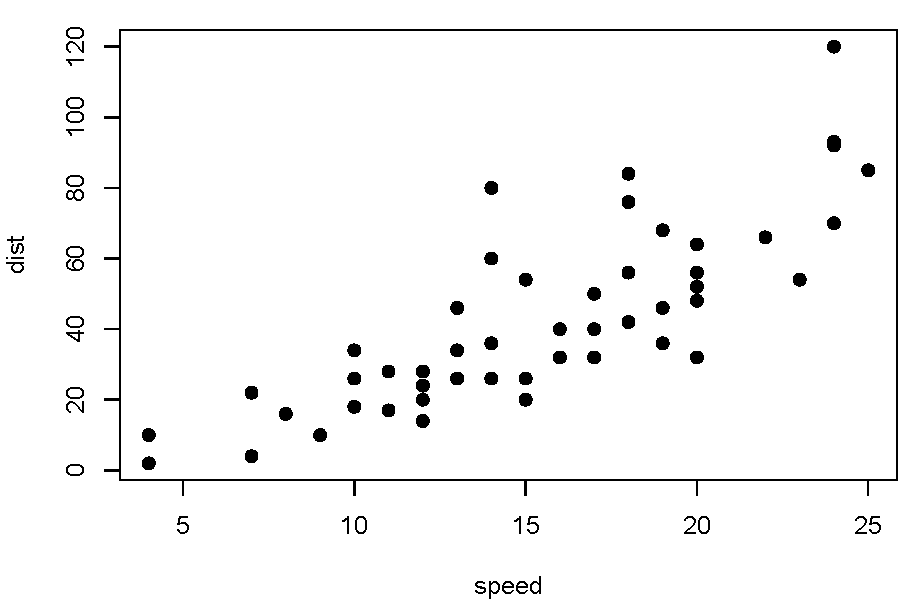
\includegraphics[width=0.9\linewidth]{bookdown_files/figure-latex/hello-1} \caption{Hello World!}\label{fig:hello}
\end{figure}

\hypertarget{cutoffs}{%
\chapter{给列变量一个阈值}\label{cutoffs}}

有时候希望获得一个剥夺矩阵\index{剥夺矩阵},具体来说,就是给列变量一个阈值\index{cutoffs},超过阈值赋值为0,低于阈值赋值1

\begin{Shaded}
\begin{Highlighting}[]
\KeywordTok{library}\NormalTok{(tidyverse)}
\KeywordTok{library}\NormalTok{(easyuse)}
\end{Highlighting}
\end{Shaded}

\begin{Shaded}
\begin{Highlighting}[]
\NormalTok{df <-}\StringTok{ }\KeywordTok{tribble}\NormalTok{(}
   \OperatorTok{~}\NormalTok{id, }\OperatorTok{~}\NormalTok{x, }\OperatorTok{~}\NormalTok{y, }\OperatorTok{~}\NormalTok{z, }\OperatorTok{~}\NormalTok{g,}
   \CommentTok{#--|--|--|--|--}
   \StringTok{"a"}\NormalTok{, }\FloatTok{13.1}\NormalTok{, }\DecValTok{14}\NormalTok{, }\DecValTok{4}\NormalTok{, }\DecValTok{1}\NormalTok{,}
   \StringTok{"b"}\NormalTok{, }\FloatTok{11.2}\NormalTok{, }\DecValTok{7}\NormalTok{, }\DecValTok{5}\NormalTok{, }\DecValTok{0}\NormalTok{,}
   \StringTok{"c"}\NormalTok{, }\FloatTok{12.5}\NormalTok{, }\DecValTok{10}\NormalTok{, }\DecValTok{1}\NormalTok{, }\DecValTok{0}\NormalTok{,}
   \StringTok{"d"}\NormalTok{, }\DecValTok{20}\NormalTok{, }\DecValTok{11}\NormalTok{, }\DecValTok{3}\NormalTok{, }\DecValTok{1}
\NormalTok{   )}
   
\NormalTok{cutoffs <-}\StringTok{ }\KeywordTok{list}\NormalTok{(}\DataTypeTok{x =} \DecValTok{13}\NormalTok{, }\DataTypeTok{y =} \DecValTok{12}\NormalTok{, }\DataTypeTok{z =} \DecValTok{3}\NormalTok{)}
\end{Highlighting}
\end{Shaded}

一般来说,可以使用 \texttt{mutate()\ +\ if\_else()}

\begin{Shaded}
\begin{Highlighting}[]
\NormalTok{df }\OperatorTok
\StringTok{  }\KeywordTok{mutate}\NormalTok{(}\DataTypeTok{x =} \KeywordTok{if_else}\NormalTok{(x }\OperatorTok{<}\StringTok{ }\NormalTok{cutoffs}\OperatorTok{$}\NormalTok{x, }\DecValTok{1}\NormalTok{, }\DecValTok{0}\NormalTok{)) }\OperatorTok
\StringTok{  }\KeywordTok{mutate}\NormalTok{(}\DataTypeTok{y =} \KeywordTok{if_else}\NormalTok{(y }\OperatorTok{<}\StringTok{ }\NormalTok{cutoffs}\OperatorTok{$}\NormalTok{y, }\DecValTok{1}\NormalTok{, }\DecValTok{0}\NormalTok{)) }\OperatorTok
\StringTok{  }\KeywordTok{mutate}\NormalTok{(}\DataTypeTok{z =} \KeywordTok{if_else}\NormalTok{(z }\OperatorTok{<}\StringTok{ }\NormalTok{cutoffs}\OperatorTok{$}\NormalTok{z, }\DecValTok{1}\NormalTok{, }\DecValTok{0}\NormalTok{))}
\end{Highlighting}
\end{Shaded}

\begin{verbatim}
## # A tibble: 4 x 5
##   id        x     y     z     g
##   <chr> <dbl> <dbl> <dbl> <dbl>
## 1 a         0     0     0     1
## 2 b         1     1     0     0
## 3 c         1     1     1     0
## 4 d         0     1     0     1
\end{verbatim}

或者使用 \texttt{pivot\_longer()} , 然后\texttt{pivot\_wider()}

\begin{Shaded}
\begin{Highlighting}[]
\NormalTok{df }\OperatorTok
\StringTok{  }\KeywordTok{pivot_longer}\NormalTok{(}\DataTypeTok{cols =}\NormalTok{ x}\OperatorTok{:}\NormalTok{z, }
               \DataTypeTok{names_to =} \StringTok{"var"}\NormalTok{, }
               \DataTypeTok{values_to =} \StringTok{"val"}\NormalTok{) }\OperatorTok
\StringTok{  }\KeywordTok{mutate}\NormalTok{(}\DataTypeTok{below_cutoff =} \KeywordTok{as.integer}\NormalTok{(val }\OperatorTok{<}\StringTok{ }\NormalTok{cutoffs[var])) }\OperatorTok\StringTok{ }
\StringTok{  }\KeywordTok{select}\NormalTok{(id, g, var, below_cutoff) }\OperatorTok
\StringTok{  }\KeywordTok{pivot_wider}\NormalTok{(}\DataTypeTok{names_from =}\NormalTok{ var, }\DataTypeTok{values_from =}\NormalTok{ below_cutoff)}
\end{Highlighting}
\end{Shaded}

\begin{verbatim}
## # A tibble: 4 x 5
##   id        g     x     y     z
##   <chr> <dbl> <int> <int> <int>
## 1 a         1     0     0     0
## 2 b         0     1     1     0
## 3 c         0     1     1     1
## 4 d         1     0     1     0
\end{verbatim}

当然,我们可以用\texttt{cutoffs\_modify\_at()}函数写的更直观一些

\begin{Shaded}
\begin{Highlighting}[]
\NormalTok{df }\OperatorTok
\StringTok{   }\KeywordTok{cutoffs_modify_at}\NormalTok{(}\DataTypeTok{.vars =} \KeywordTok{c}\NormalTok{(x, y), }\DataTypeTok{cutoffs =} \KeywordTok{c}\NormalTok{(}\DataTypeTok{x =} \DecValTok{13}\NormalTok{, }\DataTypeTok{y =} \DecValTok{12}\NormalTok{))}
\end{Highlighting}
\end{Shaded}

\begin{verbatim}
## # A tibble: 4 x 5
##   id        x     y     z     g
##   <chr> <dbl> <dbl> <dbl> <dbl>
## 1 a         0     0     4     1
## 2 b         1     1     5     0
## 3 c         1     1     1     0
## 4 d         0     1     3     1
\end{verbatim}

\hypertarget{rowwise}{%
\chapter{行方向的操作}\label{rowwise}}

tidyverse行方向的操作,喜欢用\texttt{purrr::pmap()},但遇到特殊的需求,需要写较多的语句,
比如,给指定的若干列,赋予权重,然后计算行方向的均值或者求和等等。为了简化语句增强可读性,我定义了下面一些函数

\hypertarget{ux884cux65b9ux5411ux6c42ux548c}{%
\section{行方向求和}\label{ux884cux65b9ux5411ux6c42ux548c}}

\begin{Shaded}
\begin{Highlighting}[]
\NormalTok{iris }\OperatorTok
\StringTok{   }\KeywordTok{add_row_sums}\NormalTok{(}\KeywordTok{starts_with}\NormalTok{(}\StringTok{"Sepal"}\NormalTok{), }\DataTypeTok{.name =} \StringTok{"Sepal.sum"}\NormalTok{) }\OperatorTok\StringTok{ }
\StringTok{   }\KeywordTok{head}\NormalTok{()}
\end{Highlighting}
\end{Shaded}

\begin{verbatim}
##   Sepal.Length Sepal.Width Petal.Length Petal.Width
## 1          5.1         3.5          1.4         0.2
## 2          4.9         3.0          1.4         0.2
## 3          4.7         3.2          1.3         0.2
## 4          4.6         3.1          1.5         0.2
## 5          5.0         3.6          1.4         0.2
## 6          5.4         3.9          1.7         0.4
##   Species Sepal.sum
## 1  setosa       8.6
## 2  setosa       7.9
## 3  setosa       7.9
## 4  setosa       7.7
## 5  setosa       8.6
## 6  setosa       9.3
\end{verbatim}

\hypertarget{ux884cux65b9ux5411ux6c42ux5747ux503c}{%
\section{行方向求均值}\label{ux884cux65b9ux5411ux6c42ux5747ux503c}}

\begin{Shaded}
\begin{Highlighting}[]
\NormalTok{iris }\OperatorTok
\StringTok{   }\KeywordTok{add_row_means}\NormalTok{(}\KeywordTok{starts_with}\NormalTok{(}\StringTok{"Sepal"}\NormalTok{), }\DataTypeTok{.name =} \StringTok{"Sepal.Mean"}\NormalTok{) }\OperatorTok\StringTok{ }
\StringTok{   }\KeywordTok{head}\NormalTok{()}
\end{Highlighting}
\end{Shaded}

\begin{verbatim}
##   Sepal.Length Sepal.Width Petal.Length Petal.Width
## 1          5.1         3.5          1.4         0.2
## 2          4.9         3.0          1.4         0.2
## 3          4.7         3.2          1.3         0.2
## 4          4.6         3.1          1.5         0.2
## 5          5.0         3.6          1.4         0.2
## 6          5.4         3.9          1.7         0.4
##   Species Sepal.Mean
## 1  setosa       4.30
## 2  setosa       3.95
## 3  setosa       3.95
## 4  setosa       3.85
## 5  setosa       4.30
## 6  setosa       4.65
\end{verbatim}

\hypertarget{ux884cux65b9ux5411ux8d4bux6743ux91cdux518dux6c42ux548c}{%
\section{行方向赋权重再求和}\label{ux884cux65b9ux5411ux8d4bux6743ux91cdux518dux6c42ux548c}}

\begin{Shaded}
\begin{Highlighting}[]
\KeywordTok{library}\NormalTok{(tidyverse)}
\KeywordTok{library}\NormalTok{(easyuse)}
\end{Highlighting}
\end{Shaded}

\begin{Shaded}
\begin{Highlighting}[]
\NormalTok{df <-}\StringTok{ }\KeywordTok{tribble}\NormalTok{(}
   \OperatorTok{~}\NormalTok{id, }\OperatorTok{~}\NormalTok{x, }\OperatorTok{~}\NormalTok{y, }\OperatorTok{~}\NormalTok{z, }\OperatorTok{~}\NormalTok{g,}
   \CommentTok{#--|--|--|--|--}
   \StringTok{"a"}\NormalTok{, }\FloatTok{13.1}\NormalTok{, }\DecValTok{14}\NormalTok{, }\DecValTok{4}\NormalTok{, }\DecValTok{1}\NormalTok{,}
   \StringTok{"b"}\NormalTok{, }\FloatTok{11.2}\NormalTok{, }\DecValTok{7}\NormalTok{, }\DecValTok{5}\NormalTok{, }\DecValTok{0}\NormalTok{,}
   \StringTok{"c"}\NormalTok{, }\FloatTok{12.5}\NormalTok{, }\DecValTok{10}\NormalTok{, }\DecValTok{1}\NormalTok{, }\DecValTok{0}\NormalTok{,}
   \StringTok{"d"}\NormalTok{, }\DecValTok{20}\NormalTok{, }\DecValTok{11}\NormalTok{, }\DecValTok{3}\NormalTok{, }\DecValTok{1}
\NormalTok{   )}
\NormalTok{df  }
\end{Highlighting}
\end{Shaded}

\begin{verbatim}
## # A tibble: 4 x 5
##   id        x     y     z     g
##   <chr> <dbl> <dbl> <dbl> <dbl>
## 1 a      13.1    14     4     1
## 2 b      11.2     7     5     0
## 3 c      12.5    10     1     0
## 4 d      20      11     3     1
\end{verbatim}

\begin{Shaded}
\begin{Highlighting}[]
\NormalTok{weights <-}\StringTok{ }\KeywordTok{c}\NormalTok{(}
   \DataTypeTok{x =} \FloatTok{0.25}\NormalTok{,}
   \DataTypeTok{y =} \FloatTok{0.25}\NormalTok{,}
   \DataTypeTok{z =} \FloatTok{0.25}\NormalTok{,}
   \DataTypeTok{g =} \FloatTok{0.25}
\NormalTok{ )}
\end{Highlighting}
\end{Shaded}

\begin{Shaded}
\begin{Highlighting}[]
\NormalTok{df }\OperatorTok\StringTok{ }
\StringTok{  }\KeywordTok{add_weighted_sum}\NormalTok{(x}\OperatorTok{:}\NormalTok{g, }\DataTypeTok{.name =} \StringTok{"wt_sum"}\NormalTok{, }\DataTypeTok{.weights =}\NormalTok{ weights)}
\end{Highlighting}
\end{Shaded}

\begin{verbatim}
## # A tibble: 4 x 6
##   id        x     y     z     g wt_sum
##   <chr> <dbl> <dbl> <dbl> <dbl>  <dbl>
## 1 a      13.1    14     4     1   8.02
## 2 b      11.2     7     5     0   5.8 
## 3 c      12.5    10     1     0   5.88
## 4 d      20      11     3     1   8.75
\end{verbatim}

\hypertarget{ux884cux65b9ux5411ux8d4bux6743ux91cdux518dux6c42ux5747ux503c}{%
\section{行方向赋权重再求均值}\label{ux884cux65b9ux5411ux8d4bux6743ux91cdux518dux6c42ux5747ux503c}}

\begin{Shaded}
\begin{Highlighting}[]
\NormalTok{df }\OperatorTok
\StringTok{  }\KeywordTok{add_weighted_mean}\NormalTok{(x}\OperatorTok{:}\NormalTok{g, }\DataTypeTok{.name =} \StringTok{"wt_mean"}\NormalTok{, }\DataTypeTok{.weights =}\NormalTok{ weights)}
\end{Highlighting}
\end{Shaded}

\begin{verbatim}
## # A tibble: 4 x 6
##   id        x     y     z     g wt_mean
##   <chr> <dbl> <dbl> <dbl> <dbl>   <dbl>
## 1 a      13.1    14     4     1    2.01
## 2 b      11.2     7     5     0    1.45
## 3 c      12.5    10     1     0    1.47
## 4 d      20      11     3     1    2.19
\end{verbatim}

\hypertarget{ux884cux65b9ux5411ux63a2ux6d4bux6700ux5148ux5339ux914d}{%
\section{行方向探测最先匹配}\label{ux884cux65b9ux5411ux63a2ux6d4bux6700ux5148ux5339ux914d}}

\begin{Shaded}
\begin{Highlighting}[]
\NormalTok{df <-}\StringTok{ }\KeywordTok{tibble}\NormalTok{(}
  \DataTypeTok{a =} \KeywordTok{c}\NormalTok{(}\StringTok{"b"}\NormalTok{, }\StringTok{"d"}\NormalTok{, }\StringTok{"l"}\NormalTok{, }\StringTok{"m"}\NormalTok{), }
  \DataTypeTok{x =} \KeywordTok{c}\NormalTok{(}\DecValTok{1}\NormalTok{, }\DecValTok{1}\NormalTok{, }\DecValTok{1}\NormalTok{, }\DecValTok{2}\NormalTok{), }
  \DataTypeTok{y =} \KeywordTok{c}\NormalTok{(}\DecValTok{5}\NormalTok{, }\DecValTok{1}\NormalTok{, }\DecValTok{2}\NormalTok{, }\DecValTok{3}\NormalTok{), }
  \DataTypeTok{z =} \KeywordTok{c}\NormalTok{(}\DecValTok{1}\NormalTok{, }\DecValTok{1}\NormalTok{, }\DecValTok{0}\NormalTok{, }\DecValTok{1}\NormalTok{)}
\NormalTok{)}
\NormalTok{df}
\end{Highlighting}
\end{Shaded}

\begin{verbatim}
## # A tibble: 4 x 4
##   a         x     y     z
##   <chr> <dbl> <dbl> <dbl>
## 1 b         1     5     1
## 2 d         1     1     1
## 3 l         1     2     0
## 4 m         2     3     1
\end{verbatim}

x, y, z三列,行方向选出最先大于1的值,构成新的一列

\begin{Shaded}
\begin{Highlighting}[]
\NormalTok{df }\OperatorTok\StringTok{ }\KeywordTok{mutate}\NormalTok{(}\DataTypeTok{new_col =} \KeywordTok{row_first_match}\NormalTok{(}\OperatorTok{~}\StringTok{ }\NormalTok{. }\OperatorTok{>}\StringTok{ }\DecValTok{1}\NormalTok{, x, y, z))}
\end{Highlighting}
\end{Shaded}

\begin{verbatim}
## # A tibble: 4 x 5
##   a         x     y     z new_col
##   <chr> <dbl> <dbl> <dbl>   <dbl>
## 1 b         1     5     1       5
## 2 d         1     1     1      NA
## 3 l         1     2     0       2
## 4 m         2     3     1       2
\end{verbatim}

\cleardoublepage

\hypertarget{appendix-appendix}{%
\appendix \addcontentsline{toc}{chapter}{\appendixname}}


\hypertarget{ux66f4ux591a}{%
\chapter{更多}\label{ux66f4ux591a}}

Yeah! I have finished my book, but I have more to say about some topics. Let me explain them in this appendix.

To know more about \textbf{bookdown}, see \url{https://github.com/yihui/bookdown-crc}.

  \bibliography{book.bib,packages.bib}

\backmatter
\printindex

\end{document}
